\documentclass[10pt]{article}
\usepackage{ctex}
\usepackage{CJK}
\usepackage{graphicx}
\bibliographystyle{plain}
\setlength{\parindent}{2em}
\begin{document}
\title{Stochastic resonance}
\author{Qilei Zhang}
\date{may 21 2018}
\maketitle
\par
\section{INTRODUCTION}
Noise often affects the performance of communications equipment��when the noise is too large, the input signal may be obscured and communication will be hindered. In a nonlinear system, optimizing the noise intensity can make the output signal-to-noise ratio of the system maximize, that is, generate a random resonance. In general, stochastic resonance occurs in a bistable system where weak signals and noise work together. The response of the system is driven by forces of two different time scales. The two forces coordinate with each other, making the system switch between two steady states. There is an optimized noise value that works synergistically with the force of the input signal and the output SNR can reach a maximum value. Stochastic resonance models include weak input signals, noise, and nonlinear systems for signal processing.\cite{higham1994bibtex}
\par
\begin{figure}[htbp]
\small
\centering
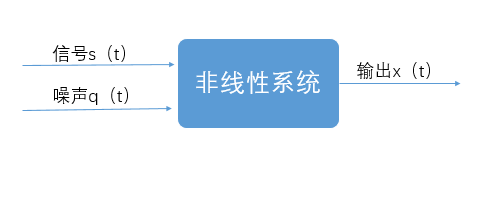
\includegraphics[width=20em]{xitong.png}
\caption{Stochastic resonance}
\label{fig:lable}
\end{figure}
\section{CHARACTERIZATION OF STOCHASTIC RESONANCE}
Stochastic resonance was quantified by the intensity of a peak in the power spectrum. Observables based on the power spectrum are indeed very convenient in theory and experiment, since they have immediate intuitive meaning and are readily measurable. First, the important quantifiers based on power spectrum stochastic resonance are discussed. With the introduction of quantifiers, we prove their properties of the two general models of stochastic resonance, periodically driven bistable two fluid system and Shuangjing system.\cite{higbibtex}
\par
The over damping motion of Brown particles in the bistable potential , under the action of noise and periodic forcing , is considered.
\par
\begin{figure}[htbp]
\small
\centering
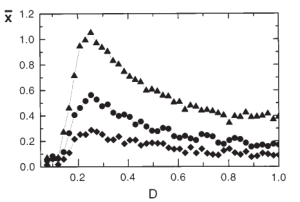
\includegraphics[width=20em]{zaosheng.png}
\caption{Typical characteristic curve of random resonance}
\label{fig:lable}
\end{figure}
\par
It can be seen in the diagram that with the increase of the noise intensity, the signal to noise ratio of the output increases greatly, and the peak value shows that there is a transfer of noise energy to the periodic signal.\cite{hibibtex}
\par
In a second part, we discuss quantifiers that are based on the interval distribution; these latter measures emphasize the synchronization aspect of stochastic resonance.
\par
SNR and SNR gain are also important indicators in stochastic resonance measure index. The resonance dependence of the amplitude X(d) of the periodic response at the noise intensity D is explained by the synchronization parameter. In the following subsection we characterize stochastic resonance as a ����resonant���� synchronization phenomenon, resulting from the combined action of noise and periodic forcing in a bistable system.
\par
\section{TOOL}
The first evidence of stochastic resonance was produced by simulating the Budyko-Sellers model of climate change  on a Digital Instruments mainframe computer , an advanced computer at the time.
\par
\section{Digital simulations}
Jung and Ha�� nggi encoded the matrix-continued fraction algorithm. Convergence problems at low noise intensities and small driving frequencies, due to the truncation procedure, are the main limitations of this algorithm.
\par
\section{Analog simulations}
Analog simulation allows more flexibility than digital simulation and for this reason has been preferred by a number of researchers. It offer some advantages: (a) a large range of parameter space can be explored rather quickly; (b) high dimensional systems may be simulated more readily than by computer.
\par
\section{Experiments}
stochastic resonance has been repeatedly observed in a large variety of experiments.
\par
\section{TWO-STATE MODEL}
we discuss the simplest model that epitomizes the class of symmetric bistable systems. For a bistable system, there are two steady states, defining n(t) as the probability that the system is at +-Xm at time t. Under the weak periodic signal s(t), the balance of the system is broken, and the bi-static potential trap periodically alternates under the action of the periodic force, and at the same time it also causes changes in the transition probability of the system output between two steady states.
\par
\section{CONTINUOUS BISTABLE SYSTEMS}
The two-state model of stochastic resonance has strict restrictions. The two-state model considers only the transitions between two steady states, and ignores the dynamic behaviors that occur during steady state and transient transitions. It is sometimes desirable to describe not only the dynamic behavior of inter-well transitions of the system but also the dynamic behavior within the potential well of the system. Therefore, the two-state model cannot be used for the random process x(t) and a more elaborate model is needed.
\par
\section{Fokker-Planck description}
we shall consider a Brownian particle of mass m that moves in a bistable potential V(x) and is subjected to thermal noise u(t) of the Nyquist type at temperature T. we perturb the particle with a periodically varying force.
\par
Langevin equation\\
$\quad mx''=-mrx'-V'(x)+mAcos(wt+c)+\sqrt{2mrkT}u(t)$\\
Here u(t) denotes a Gaussian white noise with zero average and autocorrelation function
\par
\section{Linear-response theory}
Linear-response concept and Floquet modes and the Floquet eigenvalues are are adequate methods for studying the basic physics that characterizes stochastic resonance.We shall rely on the linear-response theory and extended to the wider class of stochastic processes that admit also nonthermal, stationary nonequilibrium states.
\bibliography{abc}
\end{document}

